\documentclass{patmorin}
\usepackage{pat,graphicx,amsopn}

\newcommand{\VG}{\mathit{VG}}
\newcommand{\EVG}{\mathit{EVG}}
\newcommand{\VSP}{\mathit{VSP}}
\newcommand{\Oe}{O_\epsilon}
\DeclareMathOperator{\start}{start}


\title{\MakeUppercase{Covering Visibility Regions with Triangles:\newline
       Algorithms and Applications}}
\author{Joachim Gudmundsson\thanks{\affil{NICTA},
\email{joachim.gudmundsson@nicta.com.au}}\, 
       and Pat Morin\thanks{\affil{Carleton University},
\email{morin@scs.carleton.ca}}}

\begin{document}
\maketitle
\begin{abstract}
Let $S$ be a set of $n$ disjoint line segments in $\R^2$ and let $s$ be an
element of $S$.  A well-known example shows that the subset, $V_S(s)$, of
$\R^2$ that is weakly visible from $s$ can have complexity $\Omega(n^4)$.

In the current paper we show that $V_S(s)$ can always be covered by a set
$C_S(s)$ of $O(n^2)$ triangles.  More importantly, the expected number
of triangles needed to cover $V_S(s)$ for a random element $s\in S$ is
$O(m/n)=O(n)$ where $m=O(n^2)$ is the number of edges in the visibility
graph of $S$.

By storing sets of triangles in a version of efficient partition trees
(Matou\v{s}ek 1992), we give applications of this result to preprocessing
a segment $s\in S$ so that we can quickly determine if $s$ is visible
from a query point $p$.  We also give applications to preprocessing $S$
so that one can quickly estimate the number of segments in $S$ visible
from a query point $p$.
\end{abstract}

\section{Introduction}

Let $S$ be a set of $n$ closed line segments that are disjoint in the
sense that there are no two elements $s_1,s_2\in S$, with $s_1\neq s_2$,
such that the interior of $s_1$ and the interior of $s_2$ have a point
in common.

Two points $p,q\in\R^2$ are \emph{visible} (with respect to $S$) if the
open line segment $pq$ does not intersect any element of $S$.  A segment
$s\in S$ is \emph{visible} (with respect to $S$) from a point $p$ if there
exists a point $q\in s$ such that $p$ and $q$ are visible.  If two objects
(points, segments) $A$ and $B$ are visible (with respect to $S$), then we
say that $A$ and $B$ \emph{see} each other (with respect to $S$).

For a point $p\in\R^2$, the \emph{visibility region} or \emph{visibility
polygon} of $p$ (with respect to $S$) is defined as
\[
   V_S(p)=\{q\in\R^2:\mbox{$p$ and $q$ are visible (w.r.t. $S$)}\} 
      \enspace .
\]
The visibility region of a point is star-shaped, has $p$ in its kernel,
and has size $O(n)$. It can be computed in $O(n\log n)$ time by sorting
the endpoints of segments in $S$ radially around $p$ and then processing
these in order using a binary search tree that orders segments by the
order of their intersections with a ray emanating from $p$. (Equivalently,
one can compute the lower-envelope of $S$ in the polar coordinate
system whose origin is $p$.)  Because $V_S(p)$ is star-shaped with $p$
in its kernel it is easy to determine if a query point $q$ is contained
in $V_S(p)$ in $O(\log n)$ time using binary search. In this way, one
can consider $V_S(p)$ as an $O(n)$ sized data structure that can test,
in $O(\log n)$ time, if a query point $q$ sees $p$.

For a segment $s\in S$, the \emph{visibility region} of $s$ (with respect
to $S$)
\[
   V_S(s) = \bigcup_{q\in s} V_S(q)
          = \{p\in\R^2:\mbox{$s$ and $p$ are visible (w.r.t. $S$)} \}
\]
is the set of points in $\R^2$ that see (at least some of) $s$.
Unlike the visibility region of a point, the visibility region of a
segment is a complicated structure.  For a segment $s$, $V_S(s)$ can have
combinatorial complexity $\Omega(n^4)$ and $\R^2\setminus V_S(s)$ can
have $\Omega(n^4)$ connected components \cite[Figure~8.13]{o87}\cite[Lemma~12]{fhjmz08} (see \figref{quartic}).

More troublesome than the worst-case complexity of $V_S(s)$ is that
there there exist sets $S$ of $n$ line segments where, for most of
the elements $s\in S$, the complexity of $V_S(s)$ is $\Omega(n^2)$.
Therefore, explicitly computing $V_S(s)$ and preprocessing it for point
location does not yield a particularly space-efficient data structure
for testing if a query point $p$ sees $s$, even if $s$ is a ``typical''
(as opposed to worst-case) element of $S$

The main focus of the current paper is on methods of defining $V_S(s)$ as
the union of a small number of triangles.  In particular, we show that,
for any set $S$ of disjoint line segments, and a randomly chosen $s\in
S$, the expected number of triangles needed to cover $V_S(s)$ is $O(n)$.
This, of course, implies (and is implied by) the fact that each $V_S(s)$
can be covered by a set of triangles whose total size is $O(n^2)$.
Applications of these coverings include efficient data structures for
testing if a query point is contained in $V_S(s)$ as well as efficient
data structures for estimating the number of points of $S$ visible from
a query point.  In order to express our results more precisely, we need
some further definitions.

\subsection{Visibility Graphs and Extended Visibility Graphs}

The \emph{visibility graph} $\VG(S)$ is a graph whose vertices are the
$2n$ endpoints of the segments in $S$ and in which the edge $pq$ exists
if and only if the open line segment with endpoints $p$ and $q$ does
not intersect any (closed) segment in $S$ (see \figref{vg}.a).  It is
well-known that the number of edges $m$ of $\VG(S)$ is in $\Omega(n)\cap
O(n^2)$.  Ghosh and Mount \cite{gm91} give an optimal $O(n\log n+ m)$
time algorithm to compute the visibility graph of a set of $n$ disjoint
line segments.  Here, and throughout the remainder of the paper, $m=m(S)$
is the number of edges of $\VG(S)$.

\begin{figure}
  \begin{center}
    \begin{tabular}{cc}
    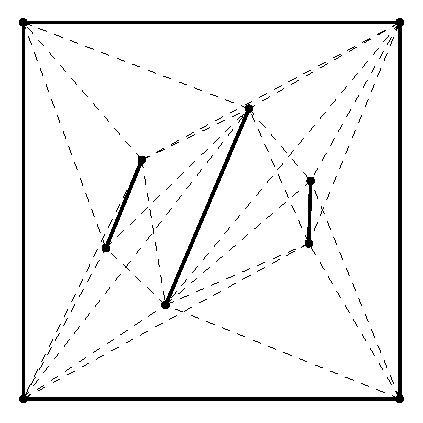
\includegraphics{vg} & 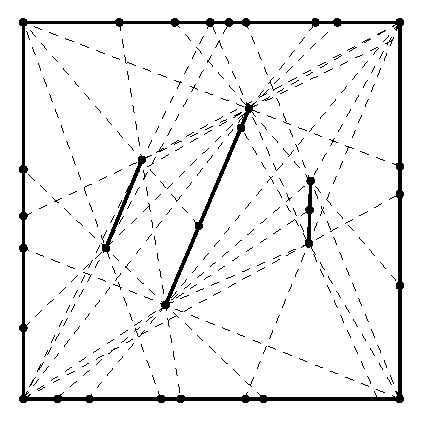
\includegraphics{evg} \\
    (a) & (b)
    \end{tabular}
  \end{center}
  \caption{The visibility graph and the extended visibility graph of a set
       of 7 line segments. (Segments are bold, graph edges are dashed.)}
  \figlabel{vg}
\end{figure}

Assume, without loss generality, that no segment in $S$ is vertical, so
we can say that a point $p$ is \emph{above} a segment $s\in S$ if $p$ is
above the line that contains $s$.  Assume, furthermore, that $S$ contains
4 segments that define a rectangle that contains all the elements of $S$
in its interior.  The first assumption can be ensured by performing a
symbolic rotation of $S$.  The second assumption is only used to ensure
that all visibility regions that we discuss are bounded.

Define the \emph{extended visibility graph} $\EVG(S)$ is obtained
by adding $2m$ edges and at most $2m$ vertices to $\VG(S)$ as follows
(see \figref{vg}.b): For each (directed) edge $uv$ in $\VG(S)$, extend a
segment $e_{uv}$ from $v$ in the direction $\overrightarrow{uv}$ until it
intersecting an element of $S$ at some point $w$.  If not already present,
then add the vertex $w$ to $\EVG(S)$ and add the edge $vw$ to $\EVG(S)$.
The extended visibility graph can be computed in $O(n\log n + m)$ time
using the visibility graph algorithm of Ghosh and Mount \cite{gm91}.

The union of the edges of $\EVG(S)$ and the segments in $S$ form a
1-dimensional set whose removal disconnects $\R^2$ into a set of
2-dimensional regions.  This set of 2-d regions is known as the
\emph{visibility space partition}, $\VSP(S)$ of $S$.  The regions
of $\VSP(S)$ are important because any region $R\in\VSP(S)$ does not
intersect the boundary of $V_S(s)$ for any element $s\in S$. That is,
for any $p,q\in R$ the set of segments of $S$ visible from $p$ is equal to
the set of segments of $S$ visible from $q$.  The region of $\VSP(S)$ that
contains $p$ determines all the combinatorial information about $V_S(p)$.

Note that $\VSP(S)$ is defined by $O(n^2)$ line segments, lines, and rays
so that it has complexity $O(n^4)$.  The example in \figref{quartic} shows
an example where this quartic complexity is achieved.

\begin{figure}
  \begin{center}
    
\includegraphics{quartic}
  \end{center}
  \caption{An example of a set $S$ where $V_S(s)$ has complexity
   $\Omega(n^4)$. The $O(n)$ segments in the center define $\Omega(n^2)$
   visibility graph edges whose extensions intersect in $\Omega(n^4)$ points.}
  \figlabel{quartic}
\end{figure}

\subsection{Previous Work}

There is a plethora of work on visibility in the plane.  This section
discusses only some of the work most relevant to the current paper.

The visibility space partition is bounded by a subset of the $O(n^2)$ lines
induced by pairs of endpoints in $S$. The arrangement of these lines can be
computed in $O(n^4)$ time using standard algorithms, and $\VSP(S)$ can be
extracted in a further $O(n^4)$ time.  This is optimal in the worst case,
since $\VSP(S)$ can have complexity $\Omega(n^4)$ \cite[Figure~8.13]{o87}
(\figref{quartic}).  More generally, $\VSP(S)$ has complexity $O(m^2)$
where $m$ is the number of edges in $\VG(S)$ and can be computed in
$O(m^2)$ time after constructing $\VG(S)$.

By preprocessing $\VSP(S)$ with a point location structure and augmenting
the regions of $S$ with appropriate information, one obtains an $O(m^2)$
size data structure that can answer the following queries:

\begin{prb}[Visibility counting]
  Given a query point $p$, report the number of segments of $S$ visible
  from $p$.  This takes $O(\log n)$ time.
\end{prb}

\begin{prb}[Visibility testing]
  Given a query point $p$ and a segment $s\in S$, determine if $p$
  sees $s$.  This takes $O(\log n)$ time.
\end{prb}

\begin{prb}[Visibility polygon construction]
  Given a query point $p$, construct the visibility polygon $V_S(p)$.
  This takes $O(m_p+\log n)$ time where $m_p=O(n)$ is the size of $V_S(p)$
  (equivalently, $m_p$ is the number of segments of $S$ visible from $p$).
\end{prb}

If the segments of $S$ are the edges of a simple polygon then Bose \etal\
\cite{blm02} and Guibas \etal\ \cite{gmr97} show that the complexity of
$\VSP(S)$ is only $O(n^3)$.  In this case, this immediately solves the
three problems above using a structure of size $O(n^3)$.  Aronov \etal\
\cite{agtz02} give a data structure that reduces the space to $O(n^2)$
but increases the $O(\log n)$ query time term to $O(\log^2 n)$, again
for the case where segments of $S$ are the edges of a simple polygon.

Pocchiola and Vegter \cite{pv96} give an $O(m)$ space data structure,
called the \emph{visibility complex} that can compute the visibility
polygon $V_S(p)$ from any query point $p$ in $O(m_p \log n)$ time,
thus giving an efficient solution to Problem~3.  Zarei and Ghodsi give
an $O(n^3)$ space data structure that can compute the visibility polygon
$V_S(p)$ in $O(m_p \log n)$ time.  More precisely, if the segments of $S$
define a polygon with $h$ holes, then the query time of their structure
is $O(\min\{h,k\}\log n + k)$, which improves the query time of Pocchiola
and Vegter when $h \ll k$.

Motivated by the computer graphics problem of estimating \emph{a priori}
the savings to be had by applying a visibility culling algorithm,
Fischer \etal\ \cite{fhjmz08,fhjmz09} give approximation algorithms for
Problem~1.  They present two approximation data structures for visibility
counting. One structure uses a $(r/m)$-cutting \cite[Section~4.5]{m02}
of $\EVG(S)$ to obtain a data structure of size $O((m/r)^2)$ that answers
queries in $O(\log n)$ time and approximates the visibility count up to
an absolute error of $r$.  Another structure uses random sampling to
obtain a data structure of size $(m^2\log^{O(1)} n)/\ell$, that has query
time $\ell\log^{O(1)} n$, and that approximates the visibility count up to
an absolute error of $\delta n$ for any constant $\delta > 0$.

\subsection{New Results}

The main result in the current paper is a proof that, for any $s\in S$,
there exists a set $C_S(s)$ of $O(m_s)$ triangles whose union is $V_S(s)$,
where $m_s$ is the number of edges of $\EVG(S)$ incident on $s$.  This
covering has an additional property that if we take the $O(m)$ size set
$C(S)=\bigcup_{s\in S}C_S(s)$ of triangles, then the number of triangles
containing any point $p\in\R^2$ is a 2-approximation to the number of
segments of $s$ that are visible from $p$.

These triangle-covering results have several applications that are
obtained by storing the resulting triangles in a layered partition tree.
Here, and throughout the remainder of the paper, $\epsilon > 0$ is a
constant that can be made arbitrarily small. To reduce clutter, we use the
notation $\Oe(f(n))=O(f(n)n^{c\epsilon})$ for some (sufficiently large,
depending on the context) constant $c$.

\subsubsection{Visibility testing} 

By storing the elements of $C_S(s)$ in a partition tree, we obtain, for
any $k$ with $m_s\le k\le m_s^2$, an $O(k)$ space data structure that can
test, in $\Oe(m_s/\sqrt{k})$ time, if a query point $p$ is contained in
$V_S(s)$.  Barring a major breakthrough on Hopcroft's Problem \cite{e96},
this result is likely only a factor of $O(n^\epsilon)$ from optimal.

For comparison purposes, the best known structure for this problem, as
used within the results of Fischer \etal\ \cite{fhjmz08,fhjmz09}, has
size $O(m_{s}^2/\ell)$ and answers queries in $O(\ell\log n)$ time, where
$\ell \ge 1$ is a space/time tradeoff parameter of the data structure.
Taking $\ell=\sqrt{n}$ yields a space of $O(m_s^{3/2})$ and a query
time of $O(\sqrt{m_s}\log n)$.  On the other hand, taking $k=m_s^{4/3}$
in our data structure yields an $O(m_s^{4/3})$ space data structure with
query time $\Oe(m_s^{1/3})$.

\subsubsection{Visibility Counting --- Absolute Approximation}

Using random sampling of the elements in $S$ in the same manner used
by Fischer \etal, we obtain a data structure of size $\Oe(m/n)=\Oe(n)$
that approximates the number of segments of $S$ visible from any query
point in time $\Oe(\sqrt{m/n})=\Oe(\sqrt{n})$ to within an absolute
error of $\delta n$ for any constant $\delta > 0$.  That is, the data
structure returns a value $m'_p$ that satisfies $m_p -\delta n \le m'_p
\le m_p+\delta n$.  (Recall that $m_p$ is the number of segments of $S$
that are actually visible from $p$.)

For comparison purposes, the cutting-based data structure of Fischer
\etal\ \cite{fhjmz08,fhjmz09}, with $r=\delta n$, uses space $O((m/n)^2)$
and has a query time of $O(\log n)$.  Using the random sampling-based
data structure of Fischer \etal\ with $\ell=\sqrt{n}$ one obtains a
data structure of size $(m^2\log^{O(1)} n)/\sqrt{n}$ with query time
$\sqrt{n}\log^{O(1)} n$.

Using random sampling in a different manner, we obtain a space versus query
time tradeoff. For any $k$ with $m/n \le k \le (m/n)^2$, we obtain a
structure of size $\Oe(k)$ and query time $\Oe((m/n)/\sqrt{k})$.  This
structure returns a visibility count $m''_p$ that satisfies $m_p-\delta n
\le m''_p \le 2m_p + \delta n$.  

\subsubsection{Visibility Counting --- Relative Approximation} 

By putting all the triangles of $C(S)$ into a partition tree, we obtain
a data structure that can $2$-approximate the number of segments of $S$
visible from any query point.  For any $k$ with $m\le k\le m^2$, this
structure has size $O(k)$ and answers queries in time $O(m/\sqrt{k})$.  The
structure returns a visibility count $m'_p$ that satisfies $m_p \le m'_p\le
2m_p$.

The remainder of the paper is organized as follows:  \Secref{covering}
proves results on covering visibility regions with triangles.
\Secref{applications} applies these results to obtain new results on
visibility testing and counting. \Secref{conclusions} summarizes and
concludes with open problems.

\section{Covering $V_S(s)$}
\seclabel{covering}

In this section we give an algorithm for covering the visibility region
$V_S(s)$ with triangles.  The number of triangles used in the covering is
bounded by $O(n+m_s)$ where $m_s$ is the number of edges of $\EVG(S)$ that
are incident to $s$.  We will show how to cover the portion
$V^+_S(s)\subseteq V_S(s)$ in the halfplane bounded from below by the
supporting line of $s$ with a set $C^+_S(s)$ of triangles.  The
complementary part $V^-_S(s)=V_S(s)\setminus V^+_S(s)$ can be covered with
a set $C^-_S(s)$ using symmetric algorithm.

The covering algorithm works by sweeping a point $p$ from left to right
across the segment $s$.  Events in this sweep occur at the vertices
$p_1,\ldots,p_{m'_s}$ of $\VSP(S)$ incident on $s$, in their left to right
order, so that $p_1$ and $p_{m'_s}$ are the left and right endpoints,
respectively, of $s$.  (Note that $m'_s \le m_s + 2$.)

Let $e$ be an edge of $V^+_S(p)$ that is collinear with $p$ and such that the
interior of $V^+_S(p)$ is to the right of $e$. We call such an edge an
\emph{active edge} of $V^+_S(p)$.  Active edges are important because, as $p$
moves to the right, they uncover regions of $\R^2$ which may not have been
previously visible.  See \figref{alg}.a.

Let $q$ be the lower endpoint of an active edge $e$ and note that $q$
is an endpoint of some segment $s\in S$. Consider what happens to $e$
as the viewpoint $p$ moves left to right along $s$, but does not cross
any edge of $\EVG(S)$ collinear with $q$.  As $p$ moves left to right,
the edge $e$ remains collinear with $p$ and $q$ and sweeps over a
triangle $\Delta_e$ whose lowest vertex is $q$.  This continues until,
at some point, the point $p$ reaches an edge of $\VSP(S)$ incident on $q$.
See \figref{alg}.b.

Algorithmically, the cover $C^+_S(s)$ is constructed as follows: Initially
$p=p_1$ is the left endpoint of $S$.  We compute the visibility polygon
$V^+_S(p)$, whose boundary is a sequence of $2m_p=O(n)$ edges that alternate
between subsegments of the elements of $S$ and segments collinear with $p$
and an endpoint of an element of $S$.  This polygon can be covered in a
natural way with $m_p$ non-overlapping triangles, each of which has $p$
as a vertex (see \figref{alg}.a). These $m_p$ triangles are added to
$C^+_S(s)$.  After computing $V^+_S(p)$ we identify its active edges, and with
each active edge $e$ we store the value $\start(e)=p_1$.

\begin{figure}
  \begin{center}
    \begin{tabular}{ccc}
      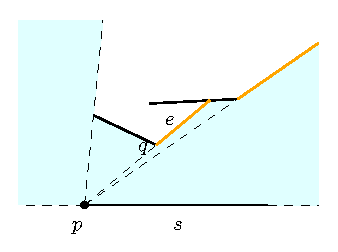
\includegraphics{alg-1} &
      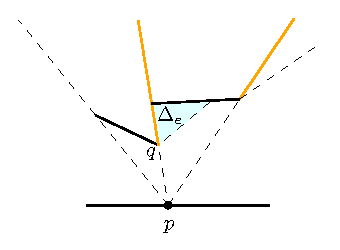
\includegraphics{alg-2} &
      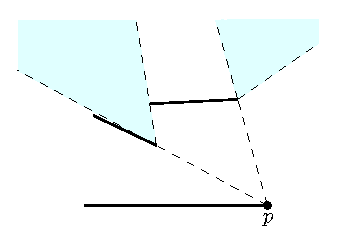
\includegraphics{alg-3} \\
      (a) & (b) & (c)
    \end{tabular}
  \end{center}
  \caption{The algorithm for covering $V^+_S(s)$ with triangles processing
           the events at (a)~$p_1$, (b)~$p_2$ and (c)~$p_3$.  
           Active edges are shown in orange and triangles in the covering
are shown at the time they are added to the covering.}
  \figlabel{alg}
\end{figure}

Next, we begin sweeping $p$ from left to right, pausing at the vertices
$p_2,\ldots,p_{m'_s}$ as we go.  Upon reaching a vertex $p_i$, we process
the edges of $\EVG(S)$ incident on $p_i$ one at a time.\footnote{For
segments in sufficiently general position, $p_i$, $1<i<m_s$ will be
incident to only one edge of $\EVG(S)$, but the covering algorithm does not
require this.}  Let $e'$ be an edge of $\EVG(S)$ incident on $p_i$. If $e'$
is collinear with an active edge $e$ of $V^+_S(p)$ then we generate a new
triangle $\Delta_e$ for $C^+_S(s)$.  The lowest vertex of $\Delta_e$ is the
lower endpoint $q$ of $e$. $\Delta_e$ is bounded by two lines
$\ell_1,\ell_2$, both of which contain $q$, and where $\ell_1$ contains
$p=p_i$ and $\ell_2$ contains $\start(e)$ .  The third side of $\Delta_e$
is bounded by the segment in $S$ incident on $e$ and furthest from $p$. See
\figref{alg}.b.

Finally, the visibility polygon $V^+_S(p)$ is updated in the neighbourhood of
$e$, which possibly creates a new active edge $f$ incident to $q$.  In this
case, $f$ is marked as active and $\start(f)=p_i$.  The exact nature of
this update depends on the relative locations of the two segments that
define $e'$.  The three possible cases are illustrated in \figref{cases}.

\begin{figure}
  \begin{center}
    \begin{tabular}{|c|c|c|}
      \includegraphics{case-a} &
      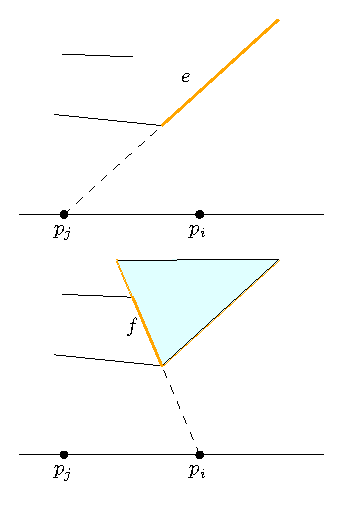
\includegraphics{case-b} &
      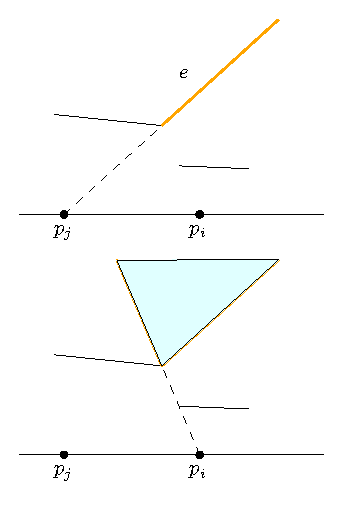
\includegraphics{case-c} \\
      (a) & (b) & (c)
    \end{tabular}
  \end{center}
  \caption{The three cases that occur when processing an edge of $\EVG(S)$
incident on $p_i$.  Here, $\start(e)=p_j$.}
  \figlabel{cases}
\end{figure}

Note that an important event, but which requires no special handling occurs
at the right endpoint of $s$ when $p=p_{m_s}$.  In this case, each active
edge of $V^+_S(p)$ generates a triangle that is added to the set $C^+_S(s)$.
See \figref{alg}.c.

We now prove the correctness of the above algorithm:

\begin{lem}\lemlabel{cover}
Let $C^+_S(s)$ be the set of triangles generated by running the above
algorithm.  Then $\cup C^+_S(s) = V^+_S(s)$ and $|C^+_S(s)|\le m_s$ where
$m_s$ is the number of edges of $\VSP(S)$ incident on $s$.
\end{lem}

\begin{proof}
To prove the bound on the size, first observe that the initial visibility
polygon $V^+_S(p_1)$ has size that is bounded by the degree of $p_1$ in
$\VSP(S)$.  Furthermore, at each event point $p_i$, $i>1$, the number of
triangles added to $C^+_S(s)$ is at most the number of edges of $\VSP(S)$
incident to $p_i$.  Therefore, the total number of triangles in $C^+_S(s)$
is at most the number of edges of $\VSP(S)$ incident to $s$.

The fact that $\cup C^+_S(s)\subseteq V^+_S(s)$ follows immediately from
the easily verifiable fact that each triangle added to $C^+_S(s)$ contains
only points visible from some point on $p\in s$.  In particular, for any
point $r$ in the triangle $\Delta_e$ that is added to $V^+_S(s)$ when
processing $p_i$, there is a point $q$ in the subsegment of $s$ between
$\start(e)$ and $p_i$ that sees $r$.

To prove that $C^+_S(s)$ covers $V^+_S(s)$, consider a point $r\in
V^+_S(s)$.  If $r$ is visible from $p_1$ then $r$ is contained in
one of the triangles added during the initialization of the algorithm.
Otherwise, there exists some point $p'\in s$ with minimum $x$-coordinate
such that $r$ is visible from $p'$.  It follows that $p'$ and $r$
are collinear with a vertex $q$ of some segment $s'\in S$ and that $q$
is on the segment $p'r$ (see \figref{cover-proof}.a).  Then $q$ is an
endpoint of an active edge $e$ of $V^+_S(p')$ with $\start(e)$ to the
left of $p'$.  Since every active edge eventually adds a triangle to
$C^+_S(s)$, there is some $p_i$ to the right of $p'$ that adds a triangle
$\Delta_e$ to $C^+_S(s)$ that contains $r$ (see \figref{cover-proof}.b).
Since this is true for every point $r\in V^+_S(s)$, we conclude that
$\cup C^+_S(s)\supseteq V^+_S(s)$, and hence $\cup C^+_S(s)= V^+_S(s)$.
\end{proof}

\begin{figure}
  \begin{center}
    \begin{tabular}{cc}
      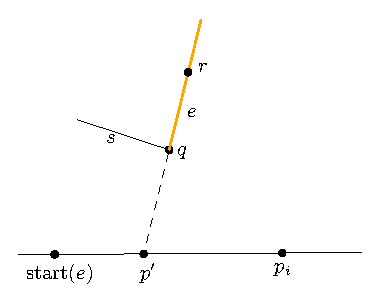
\includegraphics{cover-proof-a} &
      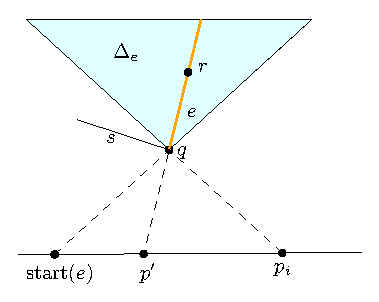
\includegraphics{cover-proof-b} \\
      (a) & (b)
    \end{tabular}
  \end{center}
  \caption{Proving that $C^+_S(s)$ covers $V^+_S(s)$.}
  \figlabel{cover-proof}
\end{figure}

Next we show that, in a global sense, the number of triangles containing a
point $p\in\R^2$ gives an approximation to the number of segments of $S$
that are visible from $p$. Let $C_S(s) = C^+_S(s)\cup C^-_S(s)$.

\begin{lem}\lemlabel{count}
Let $C(S)=\bigcup_{s\in S} C_S(s)$ and let $p$ be any point in $\R^2$ that
is not on the boundary of any triangle in $C(S)$.  If $m_p$ is the number
of segments in $S$ (partially) visible from $p$ and $m'_p$ is the number
of triangles in $C(S)$ that contain $p$, then $m_p \le m'_p \le 2m_p$.
\end{lem}

\begin{proof}
Let $C_p\subseteq C(S)$ be the set of triangles in $C(S)$ that contain
$p$, and let $S_p\subseteq S$ be the set of segments in $S$ that are
(partially) visible from $p$.  Our goal is to show that $|S_p|\le |C_p|\le
2|S_p|$. The lower bound on $m'_p=|C_p|$ is trivial: For every segment
$s\in S_p$, $V_S(s)$ contains $p$, so, by \lemref{cover}, $C_S(s)$
contributes at least one triangle to $C_p$.

To prove the upper bound, we describe a mapping $f: C_p \rightarrow S_p$
that is \emph{$2$-to-one}; for every $s\in S_p$, there exists at most 2
triangles $\Delta\in C_p$ such that $f(\Delta)=s$. The existence of $f$
then proves the upper bound.

Let $\Delta\in C_p$ be some triangle that contains $p$ and suppose that
$\Delta\in C_S(s)$ for some $s\in S$ that is, without loss of generality,
below $p$.  If $\Delta$ is incident on $s$ (\figref{counting}.a), then $\Delta$ was added to
$C_S(s)$ as part of $V_S(p)$ where $p$ was the left endpoint of $s$.  In
this case, we set $f(\Delta)=s$.  Otherwise, $\Delta$ was created when
sweeping $s$ with $p$ and some active edge $e$ of $V_S(p)$ generated
$\Delta$ (\figref{counting}.b).  The vertex $q$ of $\Delta$ that is closest to $s$ is incident on a
segment $s'\in S$.  In this case $f(\Delta)=s'$.

\begin{figure}
  \begin{center}
    \begin{tabular}{cc}
      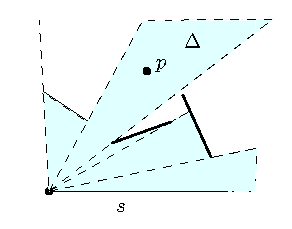
\includegraphics{counting-a} &
      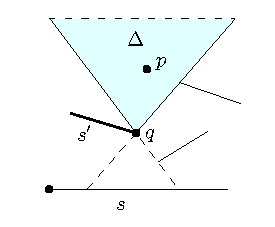
\includegraphics{counting-b} \\
      (a) $f(\Delta)=s$ & (b) $f(\Delta)=s'$
    \end{tabular}
  \end{center}
  \caption{The mapping $f$ takes $\Delta$ onto (a)~$s$ and (b)~$s'$.}
  \figlabel{counting}
\end{figure}

We now argue that $f$ is 2-to-one.  Let $s\in S$ be some segment and
suppose, without loss of generality, that $p$ is above $s$.  Consider a
triangle $\Delta \in f^{-1}(s)$ and observe that, by the definition of $f$,
$\Delta$ has a vertex that is an endpoint of $s$.

Note that there is at most one triangle in $C_S(s)\cap C_p$ that maps
to $s$, and this triangle exists precisely if $p$ is visible from the
left endpoint of $s$.  All that remains to show is that there is at
most one additional segment $s'\in S$, $s'\neq s$ such that $C_S(s')$
contains a triangle $\Delta$ with $f(\Delta)=s$.

Let $\Delta$ be such a triangle and suppose that $\Delta$ is incident to
the endpoint $q$ of $s$.  Refer to \figref{count-right}.  The triangle
$\Delta$ was generated by an active edge when processing $s'$.  In
particular, there is a subsegment $p_j p_i\subseteq s'$ such that an active
edge $e$ of $V^+_S(p)$ sweeps over $\Delta$ when $p$ travels from $p_j$ to
$p_i$. (Note, $p_j=\start(e)$.) this implies that $p_i$ and $p_j$ are below
$s$. Since $p$ travels from left to right along $e$, this implies that $q$
is the right endpoint of $s$ because, otherwise, $e$ would not be an active
edge of $V^+_S(p)$.

\begin{figure}
  \begin{center}
    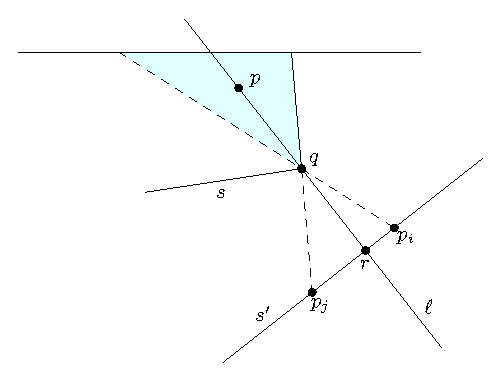
\includegraphics{count-right}
  \end{center}
  \caption{At most one triangle in $f^{-1}(s)$ is incident to the right
           endpoint of $S$.}
  \figlabel{count-right}
\end{figure}

Thus far, we have established that at most one triangle in $f^{-1}(s)$ is
incident to the left endpoint of $s$.  To see that at most one triangle
($\Delta$, discussed above) is incident to the right endpoint of $s$,
suppose by way of contradiction that there are two such triangles $\Delta$
and $\Delta'$ with $\Delta\in C_S(s')$ and $\Delta'\in C_S(s'')$.
Consider the line $\ell$ through $p$ and $q$.  Observe that $\ell$
intersects both $s$ and $s'$, in two points $r$ and $r'$, respectively. But
this is not possible since then one of $r$ or $r'$ does not see the
endpoint $q$.
\end{proof}

\paragraph{Remark:}
The condition, in \lemref{count}, that $p$ is not on the boundary of
any triangle in $C_S(s)$ is unnecessary if we take a little extra care.
In particular, the mapping $f$ actually maps triangles to the endpoints of
segments.  The set $C_S(v)$ of triangles mapped to a particular endpoint
$v$ all have $v$ as a vertex and no two triangles in $C_S(v)$ share an
interior point.  This means that we can define each triangle in $C_S(v)$
to either include or exclude some of its edges or vertices so that the
triangles are disjoint but their union remains unchanged. This yields
a set of (partially open) triangles $C'(S)$ for which \lemref{count}
holds for any point $p\in\R^2$

\section{Applications}
\seclabel{applications}

In this section, we consider applications of \lemref{cover} and
\lemref{count} to some visibility testing and counting problems. These
applications rely on data structures for \emph{triangle inclusion
counting}:  Given a set $T$ of triangles, we want to preprocess $T$
into a data structure for counting the number of triangles in $T$ that
contain a query point $p$.  The principle behind these data structures
are well-established, but finding the relevant structures and techniques,
and applying them correctly, can take some time.  Therefore, we review
the data structure here and point out the relevant references.

Let $\Delta$ be a triangle. Then $\Delta$ is the intersection of at most
4 halfplanes bounded by 4 lines $h(\Delta)=(u_1,u_2,d_1,d_2)$ where $u_1$
and $u_2$ bound $\Delta$ from below and $d_1$ and $d_2$ bound $\Delta$
from above.  (Note: in general we have either $u_1=u_2$ or $d_1=d_2$.)
By the standard duality mapping \cite[Section~8.2]{bcko08} the four lines
in $h(\Delta)$ map to four points $u_1^*$, $u_2^*$, $d_1^*$ and $d_2^*$.
A point $p\in\R^2$ maps to a line $p^*$ in the dual plane.  The point
$p$ is contained in $\Delta$ if and only if the line $p^*$ is above
(or on) $u_1^*$ and $u_2^*$ and below (or on) $d_1^*$ and $d_2^*$.
Let $h^*(\Delta)=(u_1^*,u_2^*,d_1^*,d_2^*)$.

A triangle inclusion counting structure for $T$ stores the 8-dimensional
point-set
\[
    h^*(T) = \{ h^*(\Delta) : \Delta\in T \} \enspace .
\]
Given a query point $p$, we want to count the number of points
$(a,b,c,d)\in h^*(T)$ such that satisfy the four requirements:
\begin{enumerate}
  \item $a$ is above $p^*$, and
  \item $b$ is above $p^*$, and 
  \item $c$ is below $p^*$, and
  \item $d$ is below $p^*$.
\end{enumerate}
Counting the number of points in $h^*(T)$ that satisfy any one of these
requirements is a halfplane range counting problem.  Data structures
for halfplane range counting are plentiful, and there are several
data structures known that use $\Oe(k)$ space and have query time
$\Oe(n/\sqrt{k})$ \cite[Section~4]{ae99}.  Several of these structures
(for example, Matou\v{s}ek's efficient partition trees \cite{m92}) are
hierarchical structures that are efficient and $r$-convergent (see Agarwal
and Erickson \cite[Section~5]{ae99} for definitions of hierarchical,
efficient, and $r$-convergent).  This implies \cite[Theorem~10]{ae99}
that there exists a 4-layer structure that uses $\Oe(k)$ space and
preprocessing time and that, in time $\Oe(n/\sqrt{k})$, can count the
number of elements in $h^*(T)$ that satisfy the constraints 1--4 for any
query point $p^*$.  Translating this back into primal space we obtain
the data structure we need:

\begin{thm}[\cite{m92,ae99}]\thmlabel{triangle-inclusion}
Let $T$ be a set of $n$ triangles. For any $k$ with $n\le k\le n^2$, there
exists a data structure of size $\Oe(k)$ that can be constructed in time
$\Oe(k)$ and that can count the number of triangles containing a query
point $p$ in $\Oe(n/\sqrt{k})$ time.
\end{thm}


\subsection{Visibility Testing}

Our first application follows immediately by storing the triangles of
\lemref{cover} in the data structure of \thmref{triangle-inclusion}.  This
yields our first result:

\begin{thm}\thmlabel{containment}
Let $S$ be a set of $n$ disjoint line segments and let $s\in S$
be a special segment.  For any $m_s\le k\le m_s^2$, there exists a
data structure of size $\Oe(k)$ that can test, in $\Oe(m_s/k)$ time,
if any query point $p\in\R^2$ is contained in $V_S(s)$.  Furthermore,
if we are given the $m_s$ edges of $\EVG(S)$ incident on $s$, then this
data structure can be constructed in $\Oe(k)$ time.
\end{thm}

QUESTION: Can we construct this data structure in $\Oe(k)$ time without
being given the relevant edges of $\EVG(S)$?

Next we argue that, barring a breakthrough on Hopcroft's Problem
\cite{e96}, \thmref{containment} is near-optimal.  \emph{Hopcroft's
Problem} takes as input a set $L$ of $n$ lines and a set $P$ of $n$ points
and asks if any point in $P$ is contained in any line in $L$. Currently,
the most efficient methods of solving Hopcroft's Problem have running
times in $\Omega(n^{4/3})$.  Furthermore, $\Omega(n^{4/3})$ is a lower
bound for Hopcroft's Problem in a restricted model of computation that
can model all known algorithms for the problem \cite{e96}.

Given the set $L$, we can compute the leftmost intersection point between
any pair of lines by sorting the lines by slope and checking the
intersection points between consecutive pairs of lines.  Assume, without
loss of generality, that this leftmost intersection point has
$x$-coordinate equal to 0. Using infinitesimal gaps between
segments,\footnote{The use of infinitesimals in lower bounds is justified
by Erickson's results \cite{e99b}.} we can easily construct a set of $3n+O(1)$
segments $s_0,\ldots,s_{3n+O(1)}$ such that a query point $p$ whose
$x$-coordinate is greater than 0 is visible from $s_0$ if and only if $p$
lies on one of the lines in $L$ (see \figref{hopcroft}).  For a query point
$p$ with $x$-coordinate smaller than 0 we can test if $p$ is contained in
any line of $L$ in $O(\log n)$ time by storing the lines of $L$ sorted by
slope and using binary search.

\begin{figure}
  \begin{center}
    \begin{tabular}{cc}
      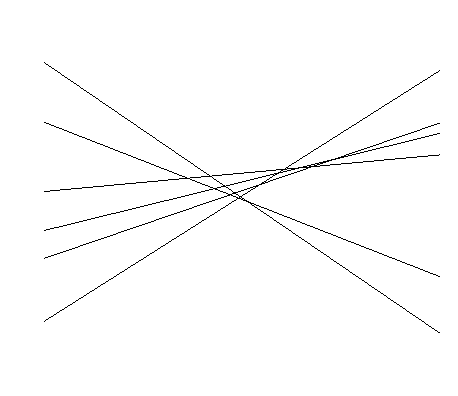
\includegraphics{hopcroft-a} &
      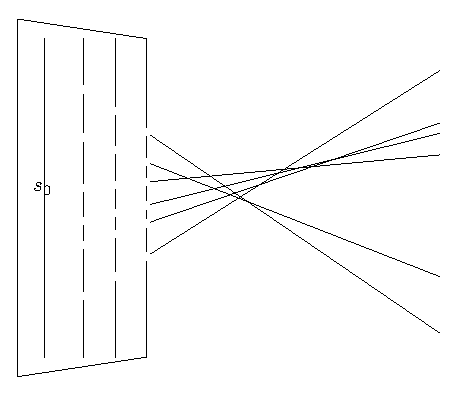
\includegraphics{hopcroft-b} \\
      (a) & (b)
    \end{tabular}
  \end{center}
  \caption{A set $L$ of lines (a) and a set of $3n+O(1)$ segments where
           testing if a point is in $V_S(s_0)$ helps to determine if
           the point is contained in any line of $L$.}
  \figlabel{hopcroft}
\end{figure}

Therefore, by the above discussion, setting $k=n^{4/3}$ and using
\thmref{containment} we can use this data structure to solve Hopcroft's
Problem in $\Oe(n^{4/3})$ time.  Furthermore, the existence of a data
structure for testing if $V_S(s)$ contains a query point $p$ that could be
constructed in $o(n^{4/3})$ time and whose query time is $o(n^{1/3})$ would
give a $o(n^{4/3})$ time algorithm for Hopcroft's Problem.

\subsection{Visibility Counting -- Absolute Approximation}

Next we consider Fischer \etal's problem of approximate visibility
counting.  We want to preprocess the segments in $S$, so that for any
query point $p$ we can quickly approximate the number of segments in $S$
that are visible from $p$.

The data structure of \thmref{containment} combined with random sampling
provides an immediate solution.  Create a Bernoulli sample $S'\subseteq
S$ by choosing each element of $S$ independently with probability
$c\log n/n$.  For each sample $s\in S'$, construct the data structure of
\thmref{containment} using $k=m_s$ that allows us to test if any query
point $p$ is visible from $s$.

Suppose $p$ is visible from $m_p$ elements of $S$, and let 
\[
   m'_p= (n/c\log n)|\{s\in S': p\in V_S(s)\}| \enspace .
\]
Then $m'_p$ is an unbiased estimator of $m_p$ and, using Chernoff's bounds
\cite[Appendix~A.1]{as08}, we readily establish that
\[
   \Pr\{|m'_p - m_p| \ge \delta n\} \le n^{-\Omega(\delta^2 c)}
\]
for any $\delta > 0$.  Thus, with high probability, $m'_p$ gives an
estimate of $m_p$ with absolute error at most $\delta n$.

All that remains is to analyze the space and query time of the resulting
data structure.  First we consider the space requirement.  The expected
amount of space that an element $s\in S$ contributes to this structure is
\[
    O\left(\frac{m_s^{1+\epsilon}c\log n}{n}\right)
\]
since it contributes $O(m_s^{1+\epsilon})$ space if it is chosen to take
part in $S'$ and it contributes nothing otherwise.  Therefore, the total
expected size of the data structure is
\begin{equation}
    \sum_{s\in S}O\left(\frac{m_s^{1+\epsilon}c\log n}{n}\right)
     = O\left(\frac{\log n}{n}\right)
         \times\sum_{s\in S}O\left(m_s^{1+\epsilon}\right)
     = O((m/n)n^{2\epsilon}\log n) \eqlabel{space-convex}
\end{equation}
where the last step follows from the fact that $\sum_{s\in S} = O(m) = O(n^2)$.

Next we analyze the query time. By the same argument used above, the
expected query time is given by 
\[
    \sum_{s\in S}O\left(\frac{m_s^{1/2+\epsilon}c\log n}{n}\right)
     = O\left(\frac{\log n}{n}\right)
         \times\sum_{s\in S}O\left(m_s^{1/2+\epsilon}\right)
     = O((m/n)^{1/2+\epsilon}\log n)
\]
where, in this case, last step follows the fact that
$f(x)=x^{1/2+\epsilon}$ is a concave function and that $\sum_{s\in S}
= O(m)$.  This gives our first result on approximate visibility counting:

\begin{thm}\thmlabel{absolute-a}
Let $S$ be a set of $n$ disjoint line segments and let $\delta > 0$ and $c>
1$ be constants.  There exists a
data structure of size $\Oe(m/n)$ that, in time $\Oe((m/n)^{1/2})$
can approximate the number of segments of $S$ visible from any query
point $p$.  With probability at least $1-n^{-\Omega(\delta^2 c)}$ the
query algorithm reports a value $m'_p$ that satisfies $m_p-\delta n \le
m'_p \le m_p+\delta n$.
\end{thm}

Unfortunately, the results of \thmref{absolute-a} become weaker if we try
to increase the space in order to decrease the query time.  The problem
comes from \eqref{space-convex} and the fact that $f(x)=x^{1+a+\epsilon}$
is convex for $a\ge 0$.  In particular, if we parameterize in terms of
the value $k$ used in the application of \thmref{containment} then we
find that the space requirement becomes $\Oe(k^2/n)$ while the query
time is $\Oe(n/\sqrt{k})$.  For example, taking $k=n^{4/3}$ gives space
$\Oe(n^{5/3})$ and query time $\Oe(n^{1/3})$.

Rather than sample segments of $S$, we instead sample triangles of $C(S)$
and use \lemref{count} to obtain a data structure of size $\Oe(k)$
that has $\Oe(n/\sqrt{k})$ query time.  The cost of this savings
in space is a weaker guarantee on the quality of the approximation
when $m_p$ is large.  Consider the set $C(S)$ of triangles described
in \lemref{count}.  For any point $p\in\R^2$, the number of triangles
$m'_p$ in $C(S)$ that contain $p$ is a 2-approximation of the number of
segments $m_p$ in $S$ that are visible from $p$.  In particular
\begin{equation}
   m_p \le m'_p \le 2m_p \enspace . \eqlabel{mpmp}
\end{equation}

Create a Bernoulli sample $C'(S)$ of $C(S)$ by sampling each triangle
in $C(S)$ with probability $c\log n / n$.  Using Chernoff's bounds, we
find that the number of triangles in $C'(S)$ is at most $O(ac(m/n)\log
n)$ with probability at least $1-n^{-\Omega(a)}$.  This concentration
result ensures that, if we put the triangles of $C'(S)$ into the
data structure of \thmref{triangle-inclusion}, then the expected
size of the structure is $\Oe(k)$ and the expected query time is
$\Oe((m/n)/\sqrt{k})$.\footnote{Actually, both the space and query time
bound hold with probability $1-n^{-\Omega(a)}$ where $a$ is the constant
hidden in the $\Oe$ notation.}

Let
\[
   m''_p= (n/c\log n)\cdot|\{\Delta\in C'(S): p\in \Delta\}| \enspace .
\]
Then $m''_p$ is an unbiased estimator of $m'_p$ that satisfies
\[
   \Pr\{|m''_p - m'_p| \ge \delta n\} \le n^{-\Omega(\delta^2 c)}
\]
for any $\delta > 0$.
Combining this with \eqref{mpmp} we obtain
\[
   \Pr\{m_p-\delta n \le m''_p \le 2m_p+\delta n\} 
     \ge 1-n^{-\Omega(\delta^2 c)}  \enspace .
\]
This gives our second result on approximate visibility counting:

\begin{thm}\thmlabel{absolute-b}
Let $S$ be a set of $n$ disjoint line segments and let $\delta > 0$ and $c
>1$ be constants.  For any $k$ with $m/n
\le k \le (m/n)^2$, there exists a data structure of size $\Oe(k)$ that,
in time $\Oe((m/n)/\sqrt{k})$ can approximately determine the number of
segments of $S$ visible from any query point $p$.  With probability at
least $1-n^{-\Omega(\delta^2 c)}$, the query algorithm
reports a value $m''_p$ that satisfies $m_p-\delta n \le m''_p \le
2m_p+\delta n$
\end{thm}

\subsection{Visibility Counting -- Relative Approximation}

Finally, we observe that by storing the $O(m)$ triangles of $C(S)$ in the
data structure of \thmref{triangle-inclusion} we obtain a data structure
that can produce relative approximations of the visibility count from any
point.

\begin{thm}\thmlabel{relative}
Let $S$ be a set of $n$ disjoint line segments. For any $k$ with
$m\le k\le m^2$,  there exists a data structure of size $k$ that can be
constructed in $\Oe(m)$ time, and can in $O(m/\sqrt{k})$ time, approximate
the number of segments of $S$ visible from any query point $p$.  The query
algorithm returns a value $m'_p$ such that $m_p \le m'_p \le 2m_p$.
\end{thm}

\section{Summary and Conclusions}
\seclabel{conclusions}

QUESTION: \thmref{absolute-a} and \thmref{absolute-b} don't consider the
construction time.  Can we build them without having to spend $O(n\log n +
m)$ time to construct the extendend visibility graph first?

We have described an algorithm for covering visibility regions with
triangles that allows several visibility testing and counting problems
to be solved using geometric range searching data structures.  These new
solutions to these problems improve considerably on the space requirements
of previous results and still provide efficient query times.

Many open questions remain.  The data structure for testing if a point is
in $V_S(s)$ for a segment $S$ (\thmref{containment}) is near-optimal,
at least assuming an $\Omega(n^{4/3})$ lower-bound for Hopcroft's
Problem.  However, it is difficult to say if the data structures for
approximate visibility counting are close to optimal.  Our solutions
reduce visibility counting to the problem of computing the depth of a
query point in an arrangement of $O((m/n)\log n)$ (\thmref{absolute-a}
and \thmref{absolute-b}) or $O(m)$ (\thmref{relative}) triangles.
In both cases, it would be sufficient to give a relative approximation
for the depth of the query point.  Unfortunately, without some additional
assumptions (such as fatness) about the triangles, there is currently
no good solution to this problem.

\section*{Acknowledgements}

This work was done while the second author was a visiting research at NICTA
and the University of Sydney.  The author is grateful for the hospitality
and funding provided by both institutions.

\bibliographystyle{plain}
\bibliography{viscover}

\end{document}
